\begin{abstract}
Machine-generated prose can show recurring lexical and syntactic choices, but a surface difference, a readable hidden direction, and a controllable behavior are not the same empirical claim. We test this distinction by following one machine--human realization signature through four increasingly demanding stages: recurrence across elicitation interfaces, cross-generator hidden-state reading, fixed-token transport, and free-generation realization. We derive the signature from matched English continuations, then test it in Llama~3.1~8B and Qwen3~4B using held-out-generator readouts and source-consistent Jacobian pullbacks. Both lexical and syntactic directions remain readable across generators. The lexical direction also produces a five-layer transport trace that exceeds every one of 100 complete fitted-pipeline nulls in both models; the syntactic direction does not. Under the tested generation protocol, however, neither direction yields reliable component-selective control. A recurrent surface signature can therefore produce fixed-token transport beyond a complete fitted-pipeline null without providing dependable control over sampled language.
% 中文：机器生成文本可能呈现反复出现的词汇和句法选择，但表面差异、可读取的隐藏方向与可控制的行为并不是同一个经验命题。我们沿着四个逐步提高要求的阶段检验同一个机器—人类语言实现特征：跨诱导接口复现、跨生成器隐藏状态读取、固定 token 传输以及自由生成实现。我们从匹配的英文续写中得到该特征，再使用留出生成器读出器和来源一致的 Jacobian 回拉，在 Llama 3.1 8B 与 Qwen3 4B 中对其进行检验。词汇和句法方向都能跨生成器读取；其中词汇方向在两个模型中都产生了超过全部 100 个完整拟合流水线零假设的五层传输轨迹，而句法方向没有。可是，在本文测试的生成协议下，两个方向都没有形成可靠的成分选择性控制。因此，反复出现的表面特征可以产生超过完整拟合流水线零假设的固定 token 传输，却不能由此提供对采样语言的可靠控制。
\end{abstract}

\begin{figure*}[t]
    \centering
    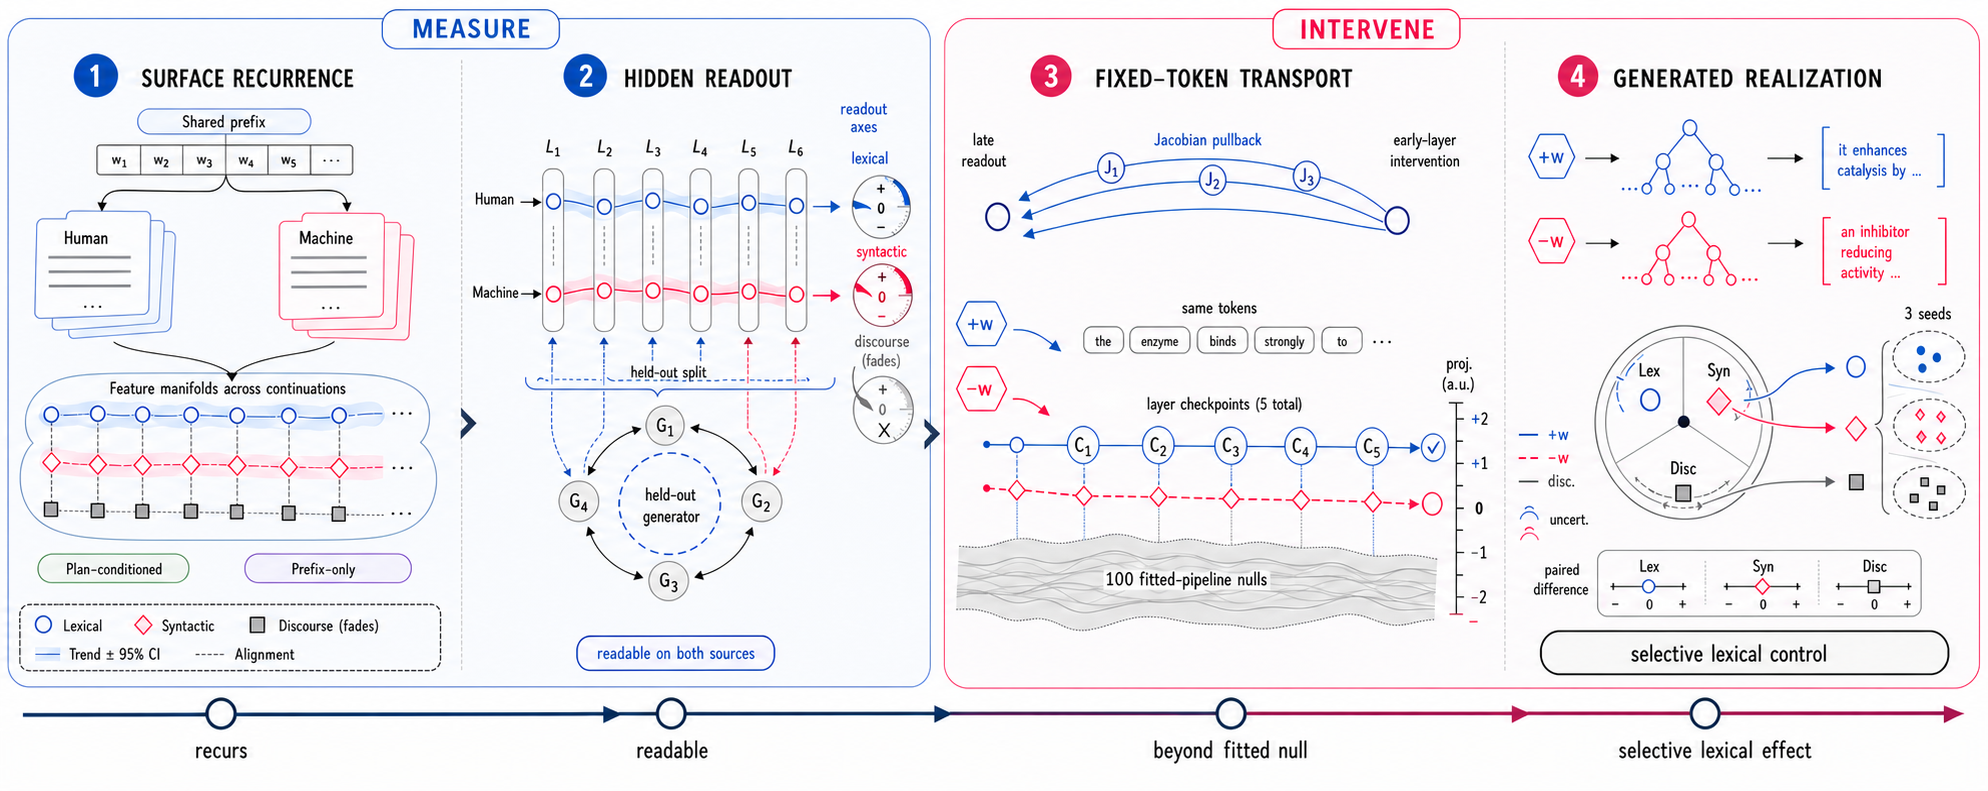
\includegraphics[width=\textwidth]{figures/main_overview.png}
    \caption{\textbf{Four tests separate recurrence, readability, transport, and realization.} Measurement fixes the surface axes and evaluates held-out readout; intervention compares fixed-token transport with 100 fitted-pipeline nulls before testing paired generations over three seeds.}
    % 中文图注：四项检验区分复现、可读取性、传输与实现。测量阶段冻结表面轴并评估留出读出；干预阶段先将固定 token 传输与 100 个拟合流水线零假设比较，再检验三个随机种子下的配对生成。
    \label{fig:main-overview}
\end{figure*}

\section{Introduction}
% 中文：引言

A human literary continuation asks, ``Why prematurely claim to have reached finality, when unexpected novelties may shatter any system before it is even completed?'' Its matched machine continuation writes, ``Claiming finality is premature because unexpected novelties can shatter any system before completion.'' The proposition is retained, but the rhetorical question becomes a declarative claim, the relation is lexicalized with \emph{because}, and function-word material is reduced. Such a pair makes a surface contrast visible. It does not tell us whether a model encodes that contrast along a common hidden direction, whether intervention transports the direction through the network, or whether the same intervention changes generated language selectively.
% 中文：一条人类文学续写写道：“既然意外的新事物可能在体系完成之前将其击碎，为什么要过早宣称体系已经终结？”与之匹配的机器续写则写道：“宣称终结为时过早，因为意外的新事物可能在体系完成之前将其击碎。”命题得以保留，但反问变成了陈述，关系由 because 明确词汇化，功能词材料也有所减少。这个例子能够直观呈现表面差异，却不能告诉我们模型是否沿共同的隐藏方向编码这种差异、干预是否会把该方向传过网络，或同一干预是否会选择性地改变生成语言。

These questions are often compressed into a single claim about ``machine-like'' text. Linguistic studies document recurrent lexical, syntactic, and rhetorical contrasts \citep{zamaraeva2025comparing,zanotto2025profiling,reinhart2025variation}; representation-based methods show that model states can reveal source or linguistic information \citep{hewitt2019probe}; and activation interventions can alter model behavior \citep{rimsky2024caa}. Each result concerns a different link. Without testing the links separately, hidden readability can be mistaken for causal transport, and transport along an unchanged trajectory can be mistaken for control over autoregressive generation.
% 中文：这些问题常被压缩成关于“机器式”文本的单一主张。语言学研究记录了反复出现的词汇、句法和修辞差异；基于表征的方法表明模型状态可以暴露来源或语言信息；激活干预也可以改变模型行为。但每类结果只对应链条中的一个环节。如果不分别检验这些环节，隐藏状态的可读性就可能被误认为因果传输，而沿不变轨迹的传输也可能被误认为对自回归生成的控制。

We study a \emph{machine--human realization signature}: a corpus-conditioned direction defined by recurrent choices of wording and clause structure while continuing the same natural context. The signature is estimated on two matched interfaces over the same 500 samples. A proposition-conditioned interface keeps machine and human content close but exposes only the machine continuation to a human-derived plan; a prefix-only interface removes that plan while permitting greater content divergence. Agreement across the interfaces makes artifacts specific to either interface less plausible, but it does not turn the signature into a universal authorship rule.
% 中文：我们研究一种“机器—人类语言实现特征”：它是在延续同一自然语境时，由反复出现的措辞和从句结构选择定义的、依赖于语料的方向。该特征在同一组 500 个样本的两个匹配接口上估计。命题条件接口使机器文本与人类文本的内容更接近，但只有机器续写会看到源自人类文本的命题计划；纯前缀接口移除了该计划，却允许更大的内容差异。两个接口之间的一致性使仅由某一接口造成的人为效应更不可信，但不会把该特征变成普适的作者身份规则。

We follow this construct through four gates (Figure~\ref{fig:main-overview}). First, the surface direction must recur across generators, domains, and the second elicitation interface. Second, a readout trained without one generator must predict the continuous surface score on both human and machine continuations from that generator. Third, a source-consistent Jacobian pullback must produce fixed-token transport beyond a null that refits the entire pipeline after breaking only the score-to-example correspondence. Fourth, the same frozen pole must yield target-aligned, component-selective effects in a separate generation experiment. The gates move from recurrence to readability, transport, and realization; passing one does not satisfy the next.
% 中文：我们让同一个构念依次通过四道检验（图~\ref{fig:main-overview}）。第一，表面方向必须在生成器、领域和第二种诱导接口之间复现。第二，在训练时排除某一生成器的读出器，必须能够预测该生成器产生的人类和机器续写中的连续表面得分。第三，来源一致的 Jacobian 回拉必须在固定 token 上产生超过完整重拟合零假设的传输，而该零假设只破坏得分与样本之间的对应关系。第四，同一个冻结极性必须在独立生成实验中产生与目标一致且具有成分选择性的效果。这四道检验依次从复现走向可读性、传输和实现；通过前一关并不能替代后一关。

Figure~\ref{fig:main-overview} links measurement to intervention without collapsing their claims. The left half fixes corpus-conditioned lexical and syntactic axes, then requires recurrence across interfaces and continuous readout on both source sides after generator holdout. The right half maps each late readout to an early intervention, compares its fixed-token trajectory with complete refitted nulls, and finally audits paired generations. The evidence narrows along this path: lexical transport crosses the fitted-null gate, syntax does not, and neither direction crosses the final selectivity gate.
% 中文：图~\ref{fig:main-overview} 将测量与干预连成一条证据链，但没有混淆二者的主张。左半部分冻结依赖于语料的词汇与句法轴，然后要求它们能够跨接口复现，并且在留出生成器后仍能在人类侧与机器侧连续读取。右半部分把每个后期读出映射为早期干预，将其固定 token 轨迹与完整重拟合零假设比较，最后审计配对生成。证据沿这条路径逐步收窄：词汇传输越过拟合零假设门槛，句法没有，而两个方向都没有越过最终的选择性门槛。

We use \emph{hidden trace} in a deliberately narrow operational sense. Readability means that the declared surface score can be recovered from hidden states; a hidden trace additionally means that an early intervention changes the corresponding late coordinate on an unchanged token trajectory beyond the fitted-pipeline null. Generated-language control is stronger still: sampled text must move along the target axis more than along off-target axes. A trace is therefore intervention evidence for coupling between tested early and late coordinates, not evidence that the coordinate is a necessary mediator of natural generation or sufficient to determine wording.
% 中文：本文有意以狭义的操作性方式使用“隐藏轨迹”这一术语。可读取性表示已声明的表面得分能够从隐藏状态中恢复；隐藏轨迹还要求早期干预在 token 轨迹不变时改变对应的后期坐标，并超过完整拟合流水线零假设。生成语言控制则更强：采样文本沿目标轴的移动必须大于沿非目标轴的移动。因此，隐藏轨迹是在所测试的早期与后期坐标之间存在耦合的干预证据，并不表示该坐标是自然生成的必要中介，也不表示它足以决定最终措辞。

The evidence narrows at the transport and generation stages. Lexical and syntactic surface directions recur and remain readable across unseen generators. Lexical fixed-token transport exceeds all 100 fitted-pipeline nulls in both target models, whereas syntactic transport remains within its null distribution despite strong directional responsiveness. Neither direction becomes reliably component-selective in free generation, and an apparent one-seed Qwen syntactic inversion changes sign across three new seeds. These results locate the boundary: a linguistic direction can recur, remain readable, and exceed a fitted-pipeline transport null without establishing control over generated language.
% 中文：证据在传输与生成阶段开始收窄。词汇和句法表面方向都能复现，并且可以在未见生成器上读取。两个目标模型中的词汇固定 token 传输都超过全部 100 个拟合流水线零假设；句法传输虽然具有很强的方向响应，却仍处于其零分布之内。两个方向在自由生成中都没有形成可靠的成分选择性，而且 Qwen 句法方向在单个种子下看似存在的反转，会在三个新种子中改变符号。这些结果定位了证据边界：一个语言方向可以反复出现、保持可读取，并超过拟合流水线传输零假设，却仍不足以建立对生成语言的控制。

Table~\ref{tab:estimands-at-glance} makes the changing evaluation unit explicit: transfer is evaluated over held-out generators, transport over fixed sequences and complete refitted pipelines, and generated-language realization over paired prompt-level effects.
% 中文：表~\ref{tab:estimands-at-glance} 明确区分了各阶段不断变化的评估单位：迁移以留出生成器评估，传输以固定序列和完整重拟合流水线评估，而生成语言实现则以提示级配对效应评估。

\begin{table*}[!tbp]
\centering
\maintablefont
\setlength{\tabcolsep}{5pt}
\renewcommand{\arraystretch}{1.10}
\begin{tabular}{@{}
  >{\raggedright\arraybackslash}p{0.12\textwidth}
  >{\raggedright\arraybackslash}p{0.16\textwidth}
  >{\raggedright\arraybackslash}p{0.64\textwidth}@{}}
\toprule
\textbf{Stage} & \textbf{Estimand} & \textbf{Construction and evaluation}\\
\midrule
Surface & Axis \(u_g\) &
500 paired feature differences; \(\Delta\), paired \(d\), and FDR \(q\).\\
Readout & Cross-generator \(D\) &
Three-generator train, one-generator test; Pearson \(r\) on both sources.\\
Pullback & Canonical \(w\) &
32 balanced Jacobian pairs; source-side agreement and frozen-anchor response.\\
Trace & Capacity \(C\) &
Five intermediate checkpoints on 100 identical fixed sequences.\\
Null test & Curve \(p_{\mathrm{null}}\) &
100 complete pipeline refits and an add-one curve-statistic rank.\\
\multirow[c]{2}{*}[-0.55ex]{Generation} & Target \(p_g\) &
Paired \(+1/-1\) generations; prompt-bootstrap target effect over 166 prompts.\\
\graycmidrule{2-3}
& Selectivity \(b_g\) &
Target response minus the mean of two off-target responses.\\
\bottomrule
\end{tabular}
\caption{\textbf{Stage-specific estimands and evaluation units.} Units progress from held-out generators to fixed sequences, refitted pipelines, and paired prompt-level effects.}
% 中文表注：各阶段使用不同的估计量与评估单位，依次从留出生成器推进到固定序列、重拟合流水线与提示级配对效应。
\label{tab:estimands-at-glance}
\end{table*}

\section{Related Work}
% 中文：相关工作

\subsection{Surface Signals}
% 中文：表面信号

Machine and human text differ in vocabulary, dependency structure, and discourse organization, although the reported cues vary across models and domains \citep{munozortiz2024contrasting,elattar2026systematic,ahmad2026human}. Detector failures under distribution shift show why these cues should not be treated as universal authorship rules \citep{sadasivan2024detection,li-etal-2024-mage,shamardina2025coat}. We instead define a corpus-conditioned multivariate direction and ask whether it recurs across named generators, domains, and elicitation interfaces.
% 中文：机器文本与人类文本在词汇、依存结构和篇章组织上存在差异，但不同模型与领域报告的线索并不一致。检测器在分布变化下的失败说明，这些线索不应被当作普适的作者身份规则。本文改为定义一个依赖于语料的多变量方向，并检验它能否在具名生成器、领域和诱导接口之间复现。

\subsection{Representation Readout}
% 中文：表征读出

Representation-based detectors can separate human and generated text from observer-model states \citep{chen-etal-2025-repreguard,vishnyakov2026svdetect}. Our readout carries a different burden: it predicts an independently measured continuous linguistic score on both sides of the source contrast, with the evaluated generator excluded from every fit. Positive human/machine agreement is required before the two source-side patterns form a consensus direction, so a source-only boundary cannot by itself satisfy the test.
% 中文：基于表征的检测器可以利用观察模型的状态区分人类文本和生成文本。本文的读出器承担不同的任务：它需要预测来源对比两侧独立测量的连续语言得分，并且被评估的生成器必须从所有拟合步骤中排除。只有在人类侧与机器侧的模式呈正向一致时，二者才能组成共识方向，因此仅仅存在来源分类边界并不足以通过检验。

\subsection{Causal Intervention}
% 中文：因果干预

Probes test whether information is accessible, whereas causal use requires intervention evidence \citep{hewitt2019probe}. Activation addition controls varied behaviors \citep{turner2023activation,rimsky2024caa,li2023iti}, but reliability depends on readout--behavior alignment, specificity, and direction identifiability \citep{canby2025reliable,waldis2026aligned,goyal2026specificity,venkatesh2026nonidentifiability}. Nullspace and amnesic methods further show that an intervention's meaning depends on the variation it removes \citep{ravfogel2020inlp,elazar2021amnesic}. Together, these literatures motivate separate tests of surface recurrence, hidden readability, fixed-token transport, and generated-language realization. We apply those tests in sequence to one fixed linguistic construct.
% 中文：探针检验信息是否可访问，而因果使用还需要干预证据。激活加法可以控制多种行为，但其可靠性取决于读出器与行为的对齐、特异性以及方向的可识别性。零空间与遗忘式方法也表明，干预的含义取决于它移除了哪类变异。综合来看，这些研究促使我们分别检验表面复现、隐藏可读性、固定 token 传输和生成语言实现；本文把这些检验依次应用于同一个固定的语言构念。

Our setting therefore sits between computational stylistics and mechanistic intervention. Surface studies supply a measurable linguistic construct, but distribution-shift failures caution against turning it into a detector; representation methods supply candidate coordinates, but accessibility alone does not establish functional use; steering methods supply an intervention, but output change must be aligned with the construct that motivated it. Keeping the same score fixed across these interfaces lets each literature contribute a distinct evidential link instead of allowing success at one link to rename the claim at the next.
% 中文：因此，本文位于计算文体学与机制干预之间。表面研究提供可测量的语言构念，但分布变化下的失败提醒我们不能把它直接变成检测器；表征方法提供候选坐标，但可访问性本身不能建立功能使用；激活引导方法提供干预，但输出变化必须与最初定义该方向的构念对齐。在这些接口之间固定同一个得分，使每类研究分别贡献一个证据环节，而不会让某一环节的成功自动改写下一环节的主张。

\section{Method}
\label{sec:method}
% 中文：方法

\subsection{Surface Signature}
\label{sec:construct}
% 中文：表面语言特征

\paragraph{Two interfaces.} The proposition-conditioned corpus contains 500 English continuation pairs balanced across PG-19, WikiLingua, Wikipedia, and XL-Sum \citep{rae2020compressive,ladhak2020wikilingua,wikimedia2023wikipedia,hasan2021xlsum}. A planner extracts a proposition plan from each human continuation, a distinct generator continues the natural prefix from that plan, and a third model checks coverage and contradiction. The prefix-only corpus regenerates the same 500 samples from the prefix and target length alone. Mean semantic cosine is 0.925 under proposition conditioning and 0.727 under prefix-only generation, compared with 0.469 after within-source derangement. The proposition-conditioned interface provides stronger content control, whereas the prefix-only interface removes the asymmetric plan-to-text channel. Section~\ref{app:corpus-detail} records construction, rejection, and leakage audits.
% 中文：两种互补接口。命题条件语料包含 500 对英文续写，并在 PG-19、WikiLingua、Wikipedia 与 XL-Sum 之间保持平衡。规划模型从每条人类续写中提取命题计划，独立的生成器依据该计划延续自然前缀，第三个模型检查内容覆盖与矛盾。纯前缀语料则只根据前缀和目标长度重新生成同一组 500 个样本。命题条件接口的平均语义余弦为 0.925，纯前缀接口为 0.727，而来源内部错配后的基线为 0.469。命题条件接口提供更强的内容控制，而纯前缀接口移除了不对称的计划到文本通道。第~\ref{app:corpus-detail} 节记录了构建、拒绝和泄漏审计。

The two arms are not interchangeable replications; they expose opposite sources of uncertainty. Proposition conditioning makes content mismatch a less plausible explanation, but the machine alone receives the explicit plan and may lexicalize its structure. Prefix-only generation removes that route, but allows larger semantic divergence. We therefore fit every axis and readout only on the proposition-conditioned arm and treat prefix-only text as an untouched transfer environment. Recurrence across the two arms cannot establish content-invariant authorship, but it is harder to attribute solely to either plan verbalization or unconstrained topic drift.
% 中文：两个分支并不是可以互换的重复实验，而是暴露了相反的不确定性来源。命题条件使内容不匹配成为较不可信的解释，但只有机器文本接收显式计划，因此可能把计划结构词汇化。纯前缀生成移除了这一路径，却允许更大的语义偏离。因此，所有轴与读出器都只在命题条件分支上拟合，纯前缀文本则作为完全未参与拟合的迁移环境。两个分支之间的复现不能建立与内容无关的作者身份，但更难仅仅归因于计划表述或无约束的主题漂移。

Sample selection is frozen before linguistic measurement. All 500 accepted proposition-conditioned pairs pass an independent automatic judge, use distinct planner, generator, and judge models, and receive no post-generation repair. Their machine--human length ratio has mean 0.935 and median 0.925, with range 0.603--1.405; length and six further nuisance statistics are nevertheless removed inside every training fold. These controls do not certify rhetorical equivalence, but they prevent the surface construct from being defined by obvious selection, repair, or length asymmetries.
% 中文：样本选择在语言测量之前冻结。全部 500 对已接受的命题条件样本都通过独立自动评审，每对都使用彼此不同的规划器、生成器与评审器，并且不进行生成后修补。机器—人类长度比的均值为 0.935，中位数为 0.925，范围为 0.603--1.405；尽管如此，长度以及另外六个干扰统计量仍在每个训练折内部被移除。这些控制不能证明修辞等价，却能避免表面构念由明显的选择、修补或长度不对称所定义。

\paragraph{Frozen directions.} We predefine 35 measurements: 10 lexical, 12 syntactic, and 13 discourse features. Seven length, entity, and number statistics are nuisance variables rather than target features. Each training fold residualizes the linguistic measurements against those nuisances, standardizes them, and projects them onto the paired machine-minus-human direction. Lexical and syntactic axes are confirmatory targets; discourse remains an off-target audit because it fails the same stability gate. The full dictionary, fold construction, PCA sensitivity, and same-token vocabulary analysis are reported in Sections~\ref{app:features} and~\ref{app:concordance}.
% 中文：冻结的语言方向。我们预先定义 35 个测量，其中包括 10 个词汇特征、12 个句法特征和 13 个篇章特征。另有 7 个长度、实体和数字统计量作为干扰变量，而不是目标特征。每个训练折先用这些干扰变量对语言测量进行残差化和标准化，再把它们投影到配对的机器减人类方向上。词汇轴和句法轴是验证性目标；篇章轴未通过相同的稳定性门槛，因此仅作为非目标审计。完整特征字典、折内构造、PCA 敏感性和同 token 词汇分析见第~\ref{app:features} 节和第~\ref{app:concordance} 节。

The construction treats the signature as a distributed relation rather than a list of diagnostic words. Grouping measurements before analysis prevents a conspicuous cue from defining the target after outcomes are known, while fold-local nuisance removal prevents length, entity density, or number density from becoming shortcuts. The paired direction then asks which combination of residualized choices changes consistently between continuations of the same context. This design makes lexical and syntactic scores interpretable as degrees of realization within the observed corpus; it does not convert any individual feature into an authorship rule.
% 中文：这一构造把该特征视为一种分布式关系，而不是诊断词汇清单。事先划分测量组，可以避免在观察结果后由某个显眼线索反过来定义目标；折内移除干扰变量，则防止长度、实体密度或数字密度成为捷径。随后，配对方向检验的是：在延续同一语境时，哪些经过残差化的语言选择组合会在人类文本与机器文本之间持续变化。因此，词汇和句法得分可以解释为观测语料内部语言实现程度的差异，但任何单个特征都不会因此成为作者身份规则。

\begin{figure*}[t]
    \centering
    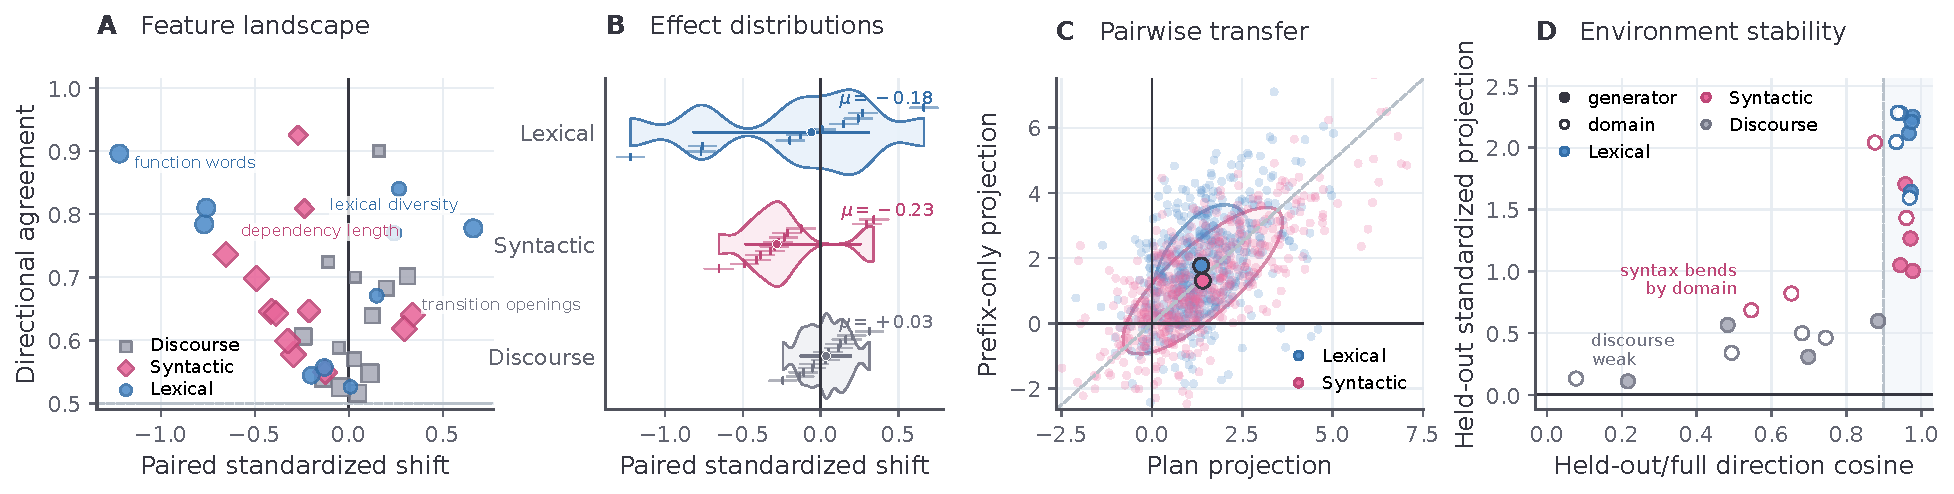
\includegraphics[width=\textwidth]{figures/machine_signature_atlas.pdf}
    \caption{\textbf{Lexical and syntactic directions recur; discourse is less stable.} (A) Frozen feature shifts and agreement. (B) Group effects. (C) Interface transfer. (D) Generator and domain holdouts.}
    % 中文图注：词汇和句法方向能够复现，篇章方向较不稳定。(A) 冻结特征位移与一致性；(B) 组级效应；(C) 接口迁移；(D) 生成器和领域留出。
    \label{fig:signature}
\end{figure*}

\subsection{Hidden Readout}
% 中文：隐藏读出

Let \(h_i^k\) be the mean continuation state after block \(k\), projected away from the leading ten pooled within-class nuisance directions. For each held-out generator and source side, we fit a forward covariance pattern between these states and the frozen surface score. Human and machine patterns must have positive cosine before their normalized sum defines the cross-generator readout \(v_g^k\). Every nuisance fit, surface direction, and hidden pattern excludes the evaluated generator. The readout is successful only if it predicts the continuous score on both human and machine continuations, rather than merely separating their sources.
% 中文：令 \(h_i^k\) 表示第 \(k\) 个模块之后的续写平均状态，并移除合并的类内干扰方向中排名最前的十个方向。针对每个留出生成器和来源侧，我们拟合隐藏状态与冻结表面得分之间的前向协方差模式。只有当人类侧和机器侧模式的余弦为正时，它们的归一化和才定义跨生成器读出方向 \(v_g^k\)。所有干扰拟合、表面方向和隐藏模式都排除被评估的生成器。读出器必须在人类续写和机器续写上都能预测连续得分，而不能只区分来源。
\begin{equation}
\begin{aligned}
\widetilde v_{ga}^k&=H_a^\top z_{ga}/(z_{ga}^\top z_{ga}), &
v_{ga}^k&=\operatorname{unit}(\widetilde v_{ga}^k),\\
v_g^k&=\operatorname{unit}(v_{g,h}^k+v_{g,m}^k), && a\in\{h,m\}.
\end{aligned}
\label{eq:covariance-readout}
\end{equation}

The readout stage tests generalization of the declared linguistic variable, not merely separability of human and machine sources. A source classifier could exploit a generator-specific artifact while remaining unrelated to the frozen realization score. Continuous prediction within both source sides instead asks whether the same hidden direction orders human and machine continuations by independently measured realization, and excluding the evaluated generator asks whether that relation survives a new generator environment. Positive held-out correlations therefore establish accessibility of the declared surface variable under generator transfer; they do not yet show that an early intervention transports it through the model.
% 中文：读出阶段检验的是已声明语言变量的泛化，而不只是人类文本与机器文本是否可分。来源分类器可能利用生成器特有的人为线索，却与冻结的语言实现得分无关。要求在人类侧和机器侧分别预测连续得分，是在检验同一个隐藏方向能否按照独立测量的语言实现程度排列两侧续写；排除被评估生成器，则检验这种关系能否迁移到新的生成器环境。因此，正的留出相关只能证明该表面变量在跨生成器条件下可访问，还不能证明早期干预会把它传过模型。

The opening literary pair also shows why an example cannot validate the readout by itself. Its machine continuation lies machineward on both frozen surface axes, yet its Llama lexical hidden difference points against the globally fitted relation. Such local reversals are compatible with a positive aggregate direction and make the held-out continuous test essential: examples interpret the construct, whereas the claim depends on ordering many unseen continuations on both source sides.
% 中文：开篇的文学样本对也说明了为什么单个例子不能独自验证读出。其机器续写在两个冻结表面轴上都位于机器方向，但其 Llama 词汇隐藏差异却与全局拟合关系相反。这样的局部反转可以与正的总体方向并存，因此留出连续检验不可或缺：具体例子负责解释构念，而经验主张依赖于在人类侧和机器侧对大量未见续写进行排序。

\subsection{Fixed-Token Transport}
% 中文：固定 token 传输

Earlier residual streams use different coordinates from the late readout. For source side \(a\), we translate the readout backward through the layer-to-layer Jacobian and combine the independently estimated human and machine pullbacks only after projecting through the frozen nuisance-nullspace projector \(P_m\):
% 中文：较早层的残差流与后期读出器使用不同坐标。对于来源侧 \(a\)，我们通过层间 Jacobian 将读出方向向前层回拉，并在经过冻结的干扰零空间投影器 \(P_m\) 后，才组合独立估计的人类侧和机器侧回拉方向：
\begin{equation}
\begin{aligned}
a_{ig}^{a}&=(J_i^{\ell\rightarrow k})^\top v_g^k,\\
\hat a^a&=\operatorname{unit}(P_m\bar a^a),\\
w_{mg}&=\operatorname{unit}(\hat a^\human+\hat a^\machine).
\end{aligned}
\label{eq:pullback-main}
\end{equation}

Applying the late readout vector directly at an early layer would assume that residual coordinates retain the same meaning across depth. The Jacobian transpose instead maps sensitivity of the declared late readout into the early residual space, so each fitted sequence contributes a local first-order pullback rather than an untransformed activation direction. Human and machine pullbacks are estimated separately, projected through the same frozen nuisance nullspace, and combined without outcome-dependent sign correction. This construction yields a preoriented early direction for the fixed-token test, but it does not optimize the surface form of sampled continuations.
% 中文：如果把后期读出向量直接施加到早期层，就等于假设残差坐标在网络深度之间保持相同含义。Jacobian 转置则把已声明后期读出器的敏感度映射回早期残差空间，使每条拟合序列贡献一个局部一阶回拉方向，而不是直接复用未经转换的激活方向。人类侧与机器侧回拉分别估计，经过同一个冻结干扰零空间投影，并且不会根据生成结果事后翻转符号。这个构造为固定 token 检验提供了预先定向的早期方向，但它并没有优化采样续写的表面形式。

The source-side signs are retained, so \(+w\) is oriented by the machineward readout before any generation outcome is observed. On an unchanged token sequence, symmetric \(+w/-w\) intervention measures the signed response of the late readout; its absolute value is the transport capacity. The confirmatory statistic is the depth-normalized area over five intermediate checkpoints, excluding the injection layer and fitted readout anchor because both are construction-internal.
% 中文：来源侧的符号保持不变，因此在观察任何生成结果之前，\(+w\) 的极性已经由机器方向的读出器确定。在不变的 token 序列上，对称的 \(+w/-w\) 干预测量后期读出器的有符号响应，其绝对值定义传输容量。验证性统计量是五个中间检查点上的深度归一化面积；注入层和拟合读出锚点都属于构造内部位置，因此被排除。
\begin{equation}
\begin{aligned}
\tau_{img}(w)&=\frac{(h_i^k(+\alpha w)-h_i^k(-\alpha w))^\top v_g^k}{2\alpha\lVert w\rVert_2},\\
\widehat C_{mgj}&=\frac{1}{n}\sum_i\lvert\tau_i(w_{mg},v_g^j)\rvert,\\
\widehat C^0_{mgj}&=\frac{1}{R}\sum_r\left[\frac{1}{n}\sum_i\lvert\tau_i(w_{mgr},v_{gr}^j)\rvert\right].
\end{aligned}
\label{eq:transport-response}
\end{equation}

The comparison is a complete fitted-pipeline null, not a random input direction. Each of \(R=100\) replicates permutes surface scores within corpus--generator strata, refits every layerwise readout, reconstructs the source-consistent pullback, and intervenes on the same 100 hashed sequences. The add-one rank \(p=(1+\#\{T_r^0\geq T\})/(R+1)\) asks whether the learned depth profile is unusual when every fitting advantage is retained but the linguistic correspondence is broken. Section~\ref{app:direction-detail} gives the complete estimands, layer conventions, trajectory checks, and sensitivity settings.
% 中文：比较对象是完整拟合流水线零假设，而不是随机输入方向。\(R=100\) 个重复中的每一个都会在语料—生成器分层内打乱表面得分，重新拟合每一层读出器，重建来源一致的回拉方向，并在相同的 100 条哈希序列上进行干预。加一排序 \(p=(1+\#\{T_r^0\geq T\})/(R+1)\) 检验：当所有拟合优势都被保留、只有语言对应关系被破坏时，学习到的深度轨迹是否仍然异常。第~\ref{app:direction-detail} 节给出完整估计量、层编号、轨迹检查与敏感性设置。

\subsection{Generated-Language Realization}
% 中文：生成语言实现

Fixed-token transport follows the response of a late readout along an unchanged trajectory. Free generation changes that trajectory as soon as the next-token distribution changes. We therefore test realization on 166 disjoint prompts, fixing poles, strengths, intervention sites, and decoding settings before observing outcomes. For measurement group \(g\), target projection \(p_{ig}\) and component selectivity \(b_{ig}\) are
% 中文：固定 token 传输沿着不变轨迹测量后期读出器的响应；自由生成则会在下一个 token 的分布发生变化时立即改变轨迹。因此，我们在 166 个互不重叠的提示上检验语言实现，并在观察结果之前冻结方向极性、强度、干预位置和解码设置。对测量组 \(g\)，目标投影 \(p_{ig}\) 与成分选择性 \(b_{ig}\) 定义如下：
\begin{equation}
\begin{aligned}
p_{ig}(w)&=s_g(Y_i^{+w})-s_g(Y_i^{-w}),\\
b_{ig}(w)&=p_{ig}(w)-\frac{1}{2}\sum_{c\neq g}p_{ic}(w).
\end{aligned}
\label{eq:selectivity}
\end{equation}
We first use a sealed one-seed matrix and eight orthonormal behavior controls for the initial audit, then evaluate the learned axes in an independent three-seed replication. Section~\ref{app:seed-detail} records the frozen 5\% norm, layer sites, token budget, temperature, top-\(p\), seeds, and prompt-clustered inference.
% 中文：我们先使用封存的单种子矩阵和八个正交行为控制完成初始审计，再用独立的三种子实验评估学习轴。第~\ref{app:seed-detail} 节记录了冻结的 5\% 范数、层位置、token 预算、温度、top-\(p\)、种子与按提示聚类的推断方法。

Target projection and component selectivity answer different questions. A direction may move its target score while shifting lexical, syntactic, and discourse measurements together, in which case the intervention changes register broadly rather than controlling the declared component. Selectivity therefore compares the target response with the mean off-target response instead of treating target movement alone as success. The sealed matrix records this cross-component structure before replication, while the independent three-seed experiment tests whether the learned-axis effect retains its direction under additional decoding randomness. A positive target interval with unresolved selectivity is accordingly evidence of target movement, not of component-selective control.
% 中文：目标投影与成分选择性回答不同问题。一个方向可能在移动自身目标得分的同时，让词汇、句法和篇章测量共同变化；此时干预改变的是整体语体，而不是对已声明成分的控制。因此，选择性需要把目标响应与非目标响应均值比较，而不能只把目标移动视为成功。封存矩阵在复现之前记录完整的跨成分响应结构，独立三种子实验则检验学习轴效应在额外解码随机性下能否保持方向。因而，目标区间为正但选择性未确定，只能作为目标发生移动的证据，不能作为成分选择性控制的证据。

\section{Experiments}
\label{sec:experiments}
% 中文：实验设置

\paragraph{Models and splits.} We evaluate hidden readout and intervention in \llamamodel{} and \qwenmodel{}. Surface axes and readouts are fitted only on the proposition-conditioned corpus. Generator transfer follows a four-fold leave-one-generator-out design, while the prefix-only corpus remains untouched until transfer evaluation.
% 中文：模型与数据划分。我们在 \llamamodel{} 和 \qwenmodel{} 中评估隐藏读出与干预。表面方向和读出器只在命题条件语料上拟合。生成器迁移采用四折留一生成器设计，纯前缀语料则在迁移评估前始终不参与拟合。

\paragraph{Evaluation protocol.} Readout is evaluated separately on held-out human and machine continuations. Fixed-token transport uses 100 identical sequences, five intermediate checkpoints, and 100 complete fitted-pipeline null refits. Generated-language realization uses 166 disjoint prompts with paired \(\pm w\) outputs, followed by an independent three-seed replication and prompt-clustered bootstrap intervals. Table~\ref{tab:estimands-at-glance} summarizes the estimands; Sections~\ref{app:direction-detail} and~\ref{app:seed-detail} give the frozen settings.
% 中文：评估协议。读出器分别在人类与机器的留出续写上评估。固定 token 传输使用 100 条完全相同的序列、五个中间检查点和 100 次完整拟合流水线零假设重拟合。生成语言实现使用 166 个互不重叠的提示生成配对的 \(\pm w\) 输出，随后进行独立的三种子复现，并使用按提示聚类的 bootstrap 区间。表~\ref{tab:estimands-at-glance} 汇总估计量；第~\ref{app:direction-detail} 节和第~\ref{app:seed-detail} 节给出冻结设置。

\section{Results}
\label{sec:results}
% 中文：结果

\begin{figure}[!t]
    \centering
    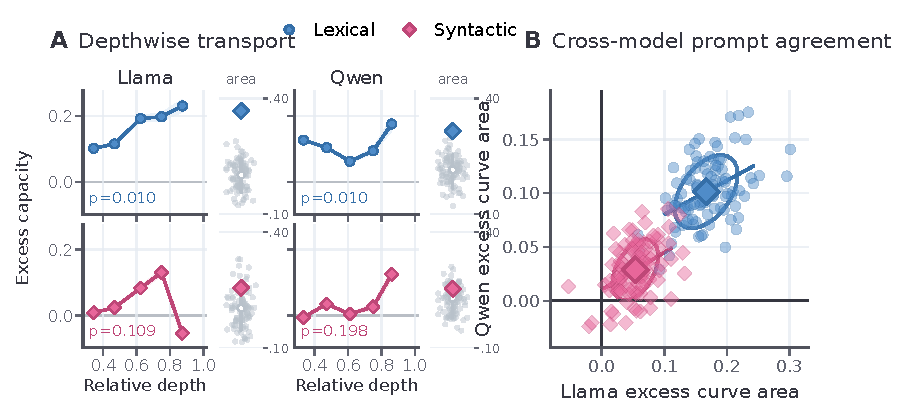
\includegraphics[width=\columnwidth]{figures/hidden_causal_trace.pdf}
    \caption{\textbf{Only lexical transport exceeds the fitted-pipeline null in both models.} (A) Five-checkpoint learned-minus-null capacity and null-ranked area. (B) Prompt-level excess area across Llama and Qwen.}
    % 中文图注：只有词汇传输在两个模型中都超过拟合流水线零假设。(A) 五检查点学习方向减零假设容量及零分布排序面积；(B) Llama 与 Qwen 的提示级超额面积。
    \label{fig:hidden-trace}
\end{figure}

\paragraph{Surface recurrence.} Figure~\ref{fig:surface-summary} separates feature magnitude from cross-environment stability. The six largest paired effects span both confirmatory groups; lexical and syntactic directions remain aligned under every generator holdout and on the untouched prefix-only corpus. All three group-level sign-flip tests yield \(p=0.0002\); prefix-only transfer is confirmatory for the lexical and syntactic axes. Syntax bends more under domain holdout, while discourse is unstable and remains off-target. Figure~\ref{fig:realization-examples} grounds the directions in paired excerpts, and Figure~\ref{fig:app-surface-transfer} reports the plan-removal transfer.
% 中文：图~\ref{fig:surface-summary} 将特征效应大小与跨环境稳定性分开呈现。最大的六个配对效应跨越两个验证性特征组；词汇和句法方向在每个生成器留出条件以及未参与拟合的纯前缀语料上都保持同向。三个组级符号翻转检验均得到 \(p=0.0002\)；纯前缀迁移只对词汇轴与句法轴进行验证性检验。句法方向在领域留出下弯曲得更多，而篇章方向不稳定，因此仍作为非目标测量。图~\ref{fig:realization-examples} 用配对摘录解释这些方向，图~\ref{fig:app-surface-transfer} 报告移除计划后的迁移。

\begin{figure}[tbp]
\centering
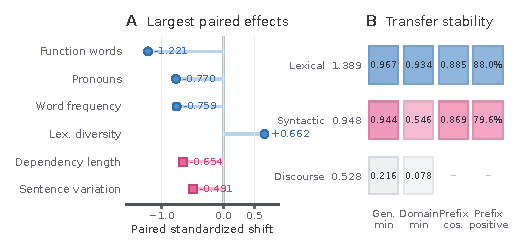
\includegraphics[width=\columnwidth]{figures/surface_result_summary.pdf}
\caption{\textbf{Surface recurrence is distributed and environment-tested.} (A) Six largest paired shifts. (B) Group shift, worst generator/domain agreement, and prefix-only transfer. Circles are lexical and squares syntactic.}
% 中文图注：表面复现具有分布式结构，并经过跨环境检验。(A) 最大的六个配对位移；(B) 组级位移、最弱生成器与领域一致性以及纯前缀迁移。圆点表示词汇特征，方块表示句法特征。
\label{fig:surface-summary}
\end{figure}

The abstract direction has visible linguistic content without reducing to a shibboleth. Across the matched corpus, \emph{however} occurs in 83 machine continuations and 34 human continuations, and \emph{despite} in 36 and 7. The evaluative forms \emph{crucial} and \emph{significant} each occur in 22 machine documents but 3 human documents; \emph{stated that} and \emph{noted that} occur in 16 and 13 machine documents and no matched human document. These counts help interpret the multivariate projection, but the direction is defined by the frozen distributed inventory rather than any one expression.
% 中文：这一抽象方向具有可见的语言内容，却不能被简化为某个刻板词汇。在匹配语料中，\emph{however} 分别出现在 83 条机器续写和 34 条人类续写中，\emph{despite} 分别为 36 与 7 条。评价性形式 \emph{crucial} 和 \emph{significant} 都出现在 22 篇机器文本中，却仅出现在 3 篇人类文本中；\emph{stated that} 与 \emph{noted that} 分别出现在 16 和 13 篇机器文本中，而未出现在任何匹配人类文本中。这些计数有助于解释多变量投影，但该方向由冻结的分布式指标库定义，而不是由任何单一表达定义。

The two transfer tests address different failure modes. Generator holdout within the proposition-conditioned arm asks whether the direction depends on one generator while content is closely matched; transfer to prefix-only outputs asks whether it persists after the human-derived plan is removed. Because prefix-only text enters neither axis construction nor readout fitting, its positive projection and readout correlation cannot result from adapting either estimator to that interface. Agreement across the arms therefore supports recurrence under two opposing content-control regimes within the environments measured here. The syntactic domain minimum of 0.546 and weaker discourse stability keep this conclusion group- and corpus-conditioned rather than universal.
% 中文：两种迁移检验针对不同的失败模式。命题条件分支中的生成器留出检验，在内容高度匹配时该方向是否依赖某一个生成器；向纯前缀输出的迁移则检验，移除源自人类文本的命题计划后该方向是否仍然存在。由于纯前缀文本既不参与轴构建，也不参与读出器拟合，其正向投影和读出相关不可能来自估计器对该接口的适配。因而，两个分支之间的一致性支持该方向在两种相反的内容控制条件下复现，但这一结论只适用于本文测量的环境。句法方向 0.546 的领域最小值以及篇章方向较弱的稳定性，进一步把结论限定在特征组和语料范围内，而不是普适规律。

\paragraph{Stable axes.} Lexical and syntactic domain-minimum cosines remain positive at 0.934 and 0.546, and 88.0\% and 79.6\% of prefix-only pairs project machineward on the original axes. The wider syntactic range shows that clause packaging is more sensitive to domain than the lexical combination, even though both transfer across generators and interfaces. Discourse behaves differently: it collapses in its weakest environments and under aggressive PCA truncation. Treating discourse as an off-target audit is therefore part of the result, not a post hoc omission of an inconvenient third axis.
% 中文：构念定义越稳定，复现也越强。词汇和句法方向在领域留出下的最小余弦仍分别为 0.934 和 0.546，纯前缀样本中分别有 88.0\% 和 79.6\% 在原始轴上投向机器方向。更宽的句法变化范围表明，从句组织比词汇组合更依赖领域，尽管两者都能跨生成器与接口迁移。篇章方向则不同：它在最弱环境与激进 PCA 截断下发生坍缩。因此，把篇章方向作为非目标审计本身就是结果的一部分，而不是事后删去一个不方便的第三轴。

\paragraph{Same-token lexical field.} A complementary analysis projects 2.44--2.48 million continuation-token states per model and compares an exact token only when it appears on both sides of a matched pair, after removing each continuation's mean coordinate. This design removes unequal token frequency and the global source offset from the local contrast. Of 612--704 eligible token contrasts per model, 89--379 survive BH-FDR together with generator and domain sign-agreement gates. The field is model- and tokenizer-specific, but it shows that the lexical direction is not exhausted by the machine side choosing a different vocabulary (Section~\ref{app:token-field}).
% 中文：共享词形内部仍然存在词汇场。一个补充分析对每个模型的 244 万至 248 万个续写 token 状态进行投影，并且只在某个完全相同的 token 同时出现在匹配样本对两侧时进行比较，同时移除每条续写的平均坐标。该设计从局部对比中移除了 token 频率不等和整体来源偏移。每个模型有 612--704 个合格 token 对比，其中 89--379 个同时通过 BH-FDR 以及生成器与领域符号一致性门控。该词汇场由模型与分词器共同决定，但它说明词汇方向并不能被完全解释为机器一侧选择了不同词汇。

\paragraph{Cross-generator readout.} All 16 held-out-generator readout observations are positive (Figure~\ref{fig:evidence-chain}A and Table~\ref{tab:readout-folds}). Mean proposition-conditioned correlations range from 0.395 to 0.450. Although no prefix-only samples enter fitting, the same readouts obtain mean correlations of 0.421--0.544 on prefix-only machine text. Human/machine pullback cosines are 0.916--0.942, whereas pullback/encoding cosines are 0.193--0.265. This difference is consistent with related but distinct encoding and pullback coordinates; it is not itself evidence of transport.
% 中文：这些方向可以跨未见生成器读取。16 个生成器留出读出观测全部为正，汇总与完整折级结果分别见图~\ref{fig:evidence-chain}A 和表~\ref{tab:readout-folds}。命题条件接口的平均相关系数为 0.395 到 0.450。虽然拟合中完全不使用纯前缀样本，同一批读出器在纯前缀机器文本上仍得到 0.421 到 0.544 的平均相关系数。人类侧与机器侧回拉余弦为 0.916 到 0.942，而回拉方向与编码方向的余弦只有 0.193 到 0.265。这种差异与相关但不同的编码和回拉坐标相一致，但其本身并不能证明传输。

\begin{table*}[!tbp]
\centering
\maintablefont
\setlength{\tabcolsep}{1.1pt}
\renewcommand{\arraystretch}{1.00}
\begin{tabular*}{\textwidth}{@{\extracolsep{\fill}}llrrrrrrrrrrr@{}}
\toprule
\multirow{2}{*}{\textbf{Held-out gen.}} & \multirow{2}{*}{\textbf{Axis}} & \multirow{2}{*}{\(\boldsymbol{\|\Delta u\|_2}\)} & \multicolumn{5}{c}{\textbf{\llamamodel} (L7\(\rightarrow\)L32)} & \multicolumn{5}{c}{\textbf{\qwenmodel} (L8\(\rightarrow\)L36)}\\
\graycmidrule{4-8}\graycmidrule{9-13}
& & & \textbf{Human \(r\)} & \textbf{Machine \(r\)} & \textbf{Mean \(r\)} & \textbf{Agree} & \textbf{Stab.} & \textbf{Human \(r\)} & \textbf{Machine \(r\)} & \textbf{Mean \(r\)} & \textbf{Agree} & \textbf{Stab.}\\
\midrule
MiniMax & Lex. & 1.473 & 0.346 & 0.464 & 0.405 & 0.519 & 0.855 & 0.355 & 0.388 & 0.372 & 0.325 & 0.939\\
DeepSeek & Lex. & 1.435 & 0.530 & 0.401 & 0.466 & 0.535 & 0.895 & 0.459 & 0.423 & 0.441 & 0.487 & 0.941\\
GLM & Lex. & 1.513 & 0.545 & 0.526 & 0.536 & 0.524 & 0.846 & 0.459 & 0.592 & 0.525 & 0.468 & 0.936\\
Qwen & Lex. & 1.213 & 0.399 & 0.392 & 0.395 & 0.486 & 0.882 & 0.432 & 0.426 & 0.429 & 0.468 & 0.925\\
\graymidrule
MiniMax & Syn. & 1.590 & 0.381 & 0.360 & 0.371 & 0.607 & 0.852 & 0.632 & 0.340 & 0.486 & 0.553 & 0.883\\
DeepSeek & Syn. & 1.453 & 0.337 & 0.446 & 0.392 & 0.433 & 0.910 & 0.445 & 0.520 & 0.483 & 0.442 & 0.910\\
GLM & Syn. & 1.429 & 0.356 & 0.396 & 0.376 & 0.576 & 0.786 & 0.496 & 0.374 & 0.435 & 0.513 & 0.914\\
Qwen & Syn. & 1.328 & 0.550 & 0.335 & 0.442 & 0.480 & 0.911 & 0.478 & 0.313 & 0.396 & 0.563 & 0.927\\
\bottomrule
\end{tabular*}
\caption{\textbf{Every held-out generator remains readable on both source sides.} Each fold trains on three generators and reports Pearson \(r\) for human and machine continuations from the fourth. Agree and Stab. denote source-side and fold/full direction cosine.}
% 中文表注：每个留出生成器在人类侧与机器侧都保持可读取。每一折使用三个生成器训练，并报告第四个生成器在人类与机器续写上的 Pearson \(r\)。Agree 与 Stab. 分别表示来源侧方向余弦以及该折与全量方向的余弦。
\label{tab:readout-folds}
\end{table*}

Readout strength, not sign, varies: source-side \(r\) ranges from 0.313 (Qwen-machine syntax under Qwen holdout) to 0.632 (Qwen-human syntax under MiniMax holdout). Fold/full cosines remain within 0.786--0.941, while human/machine agreement spans 0.325--0.607. The coordinate is therefore orientation-stable under source-side variation, supporting cross-environment readability rather than invariant effect size.
% 中文：变化发生在读出强度而非符号上：来源侧 \(r\) 从留出 Qwen 时的 Qwen 机器侧句法读出 0.313，到留出 MiniMax 时的 Qwen 人类侧句法读出 0.632。该折与全量方向的余弦保持在 0.786--0.941，而人类/机器方向一致性为 0.325--0.607。因此，在来源侧变化下，该坐标的方向仍然稳定；这支持的是跨环境可读取性，而不是不变的效应大小。

The all-positive pattern is not carried by one easy generator or one source side. Across the complete fold ledger, held-out human- and machine-side correlations range from 0.313 to 0.632, and every generator yields a positive value on both sides for both confirmatory axes. The magnitude changes with generator, source side, and axis, but the sign does not. This is the generalization needed for a consensus readout: the coordinate need not fit every environment equally well, yet it must continue to order independently measured realization after the evaluated generator is removed from every fitting step.
% 中文：全部为正的模式并不是由某一个容易的生成器或某一个来源侧支撑。在完整折级账本中，留出的人类侧与机器侧相关范围为 0.313 到 0.632，并且每个生成器在两个验证性轴的两个来源侧上都得到正值。相关强度会随生成器、来源侧和轴而变化，但符号不会改变。这正是共识读出所需的泛化：该坐标不必在所有环境中拟合得同样好，却必须在被评估生成器从所有拟合步骤中移除后，仍然能够按照独立测量的语言实现程度进行排序。

\begin{figure}[tbp]
    \centering
    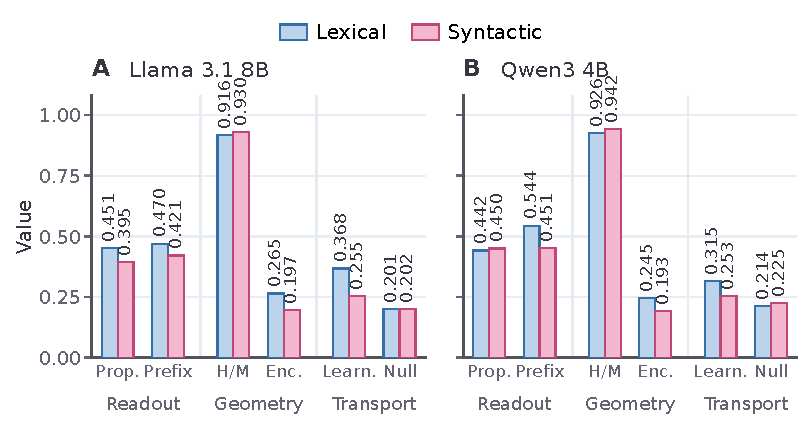
\includegraphics[width=\columnwidth]{figures/evidence_chain_summary.pdf}
    \caption{\textbf{Readout transfer and null-tested transport are distinct.} Llama (A) and Qwen (B) compare lexical and syntactic results across readout, direction alignment, and transport area.}
    % 中文图注：读出迁移与经过零假设检验的传输并不等同。Llama (A) 与 Qwen (B) 比较词汇和句法方向的读出、方向一致性与传输面积。
    \label{fig:evidence-chain}
\end{figure}

\paragraph{Lexical transport.} Llama lexical depth-normalized area is 0.368 against a null mean of 0.201; Qwen is 0.315 against 0.214. No complete null pipeline reaches either learned curve, yielding \(p=1/101=0.0099\) in both models. Learned-minus-null intervals are positive at every intermediate lexical checkpoint, and all 1,000 model--layer--sequence signed responses point machineward. This comparison preserves readout fitting, Jacobian translation, nuisance projection, and intervention trajectories; only the linguistic score-to-example correspondence is broken. The lexical effect therefore depends on that correspondence rather than on pipeline fitting alone.
% 中文：两个模型中的词汇传输都超过拟合流水线零假设。Llama 的词汇深度归一化面积为 0.368，零假设均值为 0.201；Qwen 分别为 0.315 和 0.214。没有任何完整零流水线达到两条学习曲线，因此两个模型均有 \(p=1/101=0.0099\)。每个中间词汇检查点上的学习方向减零假设区间都为正，全部 1,000 个模型—层—序列有符号响应也都指向机器方向。这一比较保留读出拟合、Jacobian 翻译、干扰投影和干预轨迹，只破坏语言得分与样本的对应关系。因此，词汇效应依赖于这一对应关系，而非仅由流水线拟合本身产生。

\paragraph{Syntactic counterexample.} Syntactic signed response points machineward in 999 of 1,000 cases, and the source-side pullbacks agree strongly. Yet its depth-normalized areas, 0.255 in Llama and 0.253 in Qwen, are reached or exceeded by 10 and 19 complete null curves, giving \(p=0.1089\) and \(p=0.1980\). One intermediate layer in each model also favors the null mean. Syntax is therefore readable and locally responsive without exceeding the fitted-pipeline transport null. The canonical pullback exceeds the construction alternatives, while nuisance-rank and fit-count variants remain close to the frozen direction (Figure~\ref{fig:app-hidden-robustness}).
% 中文：句法结果区分了方向响应与目标特异性传输。1,000 个句法有符号响应中有 999 个指向机器方向，来源两侧的回拉也高度一致。然而，Llama 和 Qwen 的句法深度归一化面积分别为 0.255 和 0.253，分别有 10 条和 19 条完整零曲线达到或超过该值，对应 \(p=0.1089\) 与 \(p=0.1980\)。每个模型中还各有一个中间层的零假设均值更高。因此，句法方向虽然可读取并具有局部方向响应，却没有超过拟合流水线传输零假设。规范回拉超过构造替代方向，而干扰秩与拟合样本数变体仍接近冻结方向，详见图~\ref{fig:app-hidden-robustness}。

The lexical--syntactic contrast is more informative than either signed-response count alone because both axes pass the same surface and readout gates and enter the same intervention pipeline. If expected orientation or frequent local response were sufficient, syntax would appear nearly as strong as lexical realization. The fitted-pipeline null changes that interpretation: every complete refit remains below the lexical curve in both models, whereas 10 Llama and 19 Qwen null curves reach or exceed the syntactic statistic. Lexical transport therefore depends on the learned score-to-example correspondence; syntax marks the limit of treating directional responsiveness as target-specific transport.
% 中文：词汇与句法之间的对比比任何单独的有符号响应计数更有信息，因为两个方向都通过了相同的表面与读出检验，并进入同一套干预流水线。如果预期极性或频繁的局部响应已经足以构成证据，那么句法方向看起来几乎会与词汇方向同样强。完整拟合流水线零假设改变了这一解释：两个模型中的全部完整重拟合都低于词汇曲线，而 Llama 的 10 条和 Qwen 的 19 条零曲线达到或超过句法统计量。因此，词汇传输依赖于学习到的得分—样本对应关系；句法结果则标出了把方向响应等同于目标特异性传输的边界。

\paragraph{Construction robustness.} In all four model--axis cases, the canonical pullback has greater five-checkpoint capacity than upstream encoding, raw and nuisance-nullspace source contrasts, and the projected-random ensemble. Nuisance-rank and Jacobian-fit-count variants remain close to the frozen direction. These checks support a source-consistent pullback over simpler substitutes; the complete refitted null still determines the lexical headline result (Figure~\ref{fig:app-hidden-robustness}).
% 中文：在四个模型—轴组合中，规范回拉的五检查点容量都高于上游编码、原始来源对比、干扰零空间来源对比以及投影随机集合。干扰秩与 Jacobian 拟合样本数变体也保持接近冻结方向。这些检查支持采用来源一致回拉而不是更简单的替代方向；决定词汇主结果的仍然是完整重拟合零假设，详见图~\ref{fig:app-hidden-robustness}。

\begin{figure}[!t]
    \centering
    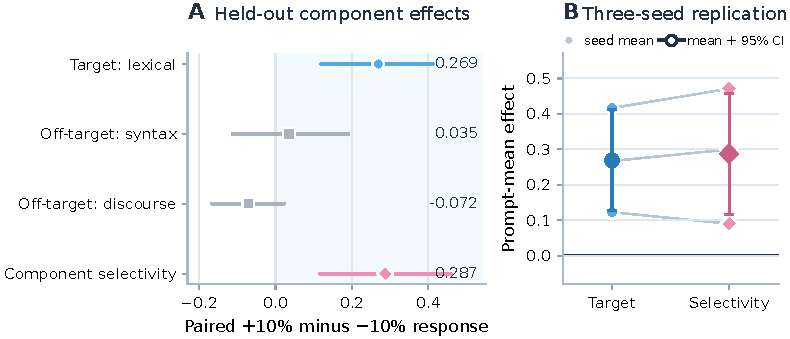
\includegraphics[width=\columnwidth]{figures/representation_realization_audit.pdf}
    \caption{\textbf{Generated-language effects are seed-sensitive and not reliably selective.} (A) Held-out readout and sealed response matrices. (B) Three-seed target projection and selectivity; points are seed means.}
    % 中文图注：生成语言效应对随机种子敏感，且没有表现出可靠选择性。(A) 留出读出与封存响应矩阵；(B) 三种子目标投影与选择性，小点表示种子均值。
    \label{fig:audit}
\end{figure}

\begin{table}[tbp]
\centering
\maintablefont
\setlength{\tabcolsep}{2.1pt}
\renewcommand{\arraystretch}{1.08}
\begin{tabular*}{\columnwidth}{@{\extracolsep{\fill}}llrr@{}}
\toprule
\textbf{Model} & \textbf{Axis} & \shortstack{\textbf{Target projection}\\\textbf{[95\% CI]}} & \shortstack{\textbf{Selectivity}\\\textbf{[95\% CI]}}\\
\midrule
\multirow[c]{2}{*}{\shortstack[l]{Llama 3.1\\8B}} & Lex. & 0.123 [\textminus0.010, 0.255] & 0.139 [\textminus0.049, 0.345]\\
\graycmidrule{2-4}
& Syn. & \textbf{0.249 [0.043, 0.518]} & 0.152 [\textminus0.092, 0.445]\\
\graymidrule
\multirow[c]{2}{*}{\shortstack[l]{Qwen3\\4B}} & Lex. & 0.012 [\textminus0.169, 0.195] & 0.027 [\textminus0.181, 0.234]\\
\graycmidrule{2-4}
& Syn. & 0.025 [\textminus0.189, 0.295] & 0.029 [\textminus0.221, 0.315]\\
\bottomrule
\end{tabular*}
\caption{\textbf{Target movement does not imply component selectivity.} Entries are prompt-clustered three-seed means with 95\% bootstrap intervals over 166 prompts; every selectivity interval includes zero.}
% 中文表注：目标移动并不意味着成分选择性。表中为 166 个提示上的提示聚类三种子均值及 95\% bootstrap 区间；所有选择性区间都包含零。
\label{tab:generation-audit}
\end{table}

\paragraph{Generation audit.} Table~\ref{tab:generation-audit} distinguishes target movement from selectivity. Only Llama syntax has a positive target interval, and none of the four conditions has resolved selectivity. Qwen syntax seed means change from \(-0.245\) and \(-0.064\) to \(+0.384\). Seven of eight pairwise selectivity intervals also include zero. Paired semantic similarity remains 0.864--0.875; prompt distributions and guardrails appear in Figure~\ref{fig:app-generation-robustness}.
% 中文：表~\ref{tab:generation-audit} 区分了目标移动与成分选择性。只有 Llama 句法方向具有正的目标区间，而四个条件都没有得到确定的选择性区间。Qwen 句法方向的种子均值从 \(-0.245\) 和 \(-0.064\) 变为 \(+0.384\)。八个成对选择性区间中还有七个包含零。配对语义相似度保持在 0.864 到 0.875；提示分布与保护指标见图~\ref{fig:app-generation-robustness}。

\section{Discussion}
% 中文：讨论

\paragraph{Evidence boundary.} Lexical realization passes recurrence, unseen-generator readout, and fixed-token transport beyond the complete fitted-pipeline null. Syntax shows why the third test matters: its readout transfers and nearly every signed response has the expected orientation, yet its transport profile remains typical of the null. The generation audit sets a stronger requirement because a transported coordinate must also survive sampling and move its target more than off-target components. Accessibility and local response therefore do not establish control.
% 中文：词汇语言实现依次通过跨环境复现、未见生成器读出以及超过完整拟合流水线零假设的固定 token 传输。句法方向说明了第三项检验为何必要：它的读出能够迁移，几乎所有有符号响应也具有预期方向，但其传输轨迹仍然处于零分布内。生成审计提出了更强要求，因为被传输的坐标还必须经受采样，并且对目标成分的移动大于非目标成分。因此，可访问性与局部响应都不能建立控制主张。

\paragraph{Evaluation rule.} Fixed-token pullback and free generation follow different gradients. Qwen's seed reversal and Llama's positive but nonselective syntactic response are consistent with this mismatch, although the experiments do not identify a single mechanism. Steering claims should therefore pair an end-to-end fitted null with a replicated generation audit of target movement, off-target response, and prompt heterogeneity. Token-conditional, multi-layer, and behavior-gradient-aware controllers remain separate estimands rather than explanations supplied by the present data.
% 中文：固定 token 回拉与自由生成遵循不同梯度。Qwen 的种子反转以及 Llama 句法方向为正但不具选择性的响应，与这种不匹配相一致，但本文实验并未识别出单一机制。因此，激活引导主张应同时使用端到端拟合零假设与复现生成审计，并联合评估目标移动、非目标响应与提示异质性。token 条件、多层和行为梯度感知控制器属于独立估计对象，而不是当前数据已经给出的解释。

\section{Conclusion}
% 中文：结论

We traced one frozen machine--human realization signature from surface recurrence through hidden readout and fixed-token transport to generated language. Lexical and syntactic directions recur across four generators and two interfaces and remain readable under generator holdout. Lexical transport exceeds all 100 complete fitted-pipeline nulls in both models, with \(p=0.0099\); syntax does not despite near-universal directional response. In generation, all component-selectivity intervals include zero, and the Qwen syntactic effect changes sign across seeds. These results separate readability, matched transport, and selective realization: coupling on a controlled trajectory does not establish dependable control over sampled language.
% 中文：本文沿表面复现、隐藏读出、固定 token 传输与生成语言，追踪同一个冻结的机器—人类语言实现特征。词汇和句法方向能够跨四个生成器和两个接口复现，并在生成器留出条件下保持可读取。词汇传输在两个模型中都超过全部 100 个完整拟合流水线零假设，\(p=0.0099\)；句法方向虽然几乎总是产生预期方向的响应，却没有超过零假设。在生成中，所有成分选择性区间都包含零，Qwen 的句法效应还会跨随机种子改变符号。这些结果区分了可读取性、匹配传输与选择性实现：受控轨迹上的耦合并不能建立对采样语言的可靠控制。
